\chapter{Single-Agenten Tasks}
\label{chap:single-tasks}
Um die Auswirkungen verschiedener Trainingsszenarien sowie die jeweils nötigen Anpassungen zu untersuchen, wurden mehrere spezifische Tasks erstellt. Die zentrale Aufgabe des Agenten besteht darin, sein Überleben zu sichern, indem er rechtzeitig eine Futterquelle findet und aufbraucht, bevor er vom Jäger gefangen wird. Diese Aufgabe lässt sich hier in drei einfachere Aufgaben aufteilen. Diese unterscheiden sich im Aufbau der Karte, Rewardfunktion sowie der spezifischen Hilfsvektoren, den sie als Observation erhalten. Die Tasks haben ebenfalls unterschiedliche Terminationsvoraussetzungen für die Trainingsepisoden.

\section{Task 1: Navigation}
\subsection{Methodik}
Task 1 stellt dem Agenten die Aufgabe, zur Position eines bekannten Zielpunkts zu navigieren. Der Agent erhält als Hilfsvektor die Richtung und Distanz zum Zielpunkt, auch wenn dieser sich nicht im Sichtfeld des Agenten befindet. Die Episode endet, wenn der Agent sich innerhalb eines bestimmten Radius vom Ziel befindet. 

\begin{figure}[htbp]
  \centering
  \adjincludegraphics[
     width=0.8\linewidth,
     Clip={0 {0\height} 0 {0.1\height}} 
  ]{Bilder/navigate.png}
  \caption{Navigation}
  \label{fig:navigate_scenario}
\end{figure}

Für das Training des Modells wurden mehrere Parameter und Rewardfunktionen getestet. In der ersten Variante erhielt der Agent eine negative Belohnung für jeden Kontakt mit Wänden und Hindernissen, und eine positive Reward für das annähern an den Zielpunkt. Diese wurde durch die Differenz der Distanz $D_t$ zum Ziel zur Distanz $D_t-1$ zum Ziel im vorherigen Schritt berechnet. In der angepassten Version wurde die Strafe für Wandkollisionen so modifiziert, dass sie mit abnehmendem Abstand zur Wand stärker ausfällt, wodurch ein abrupter Abfall der Belohnung vermieden wird. Ebenfalls wurde die Belohnung für die Distanzänderung zum Ziel so gestaltet, das diese nicht-linear ansteigt. Die letzten Schritte zum Ziel hin beziehungsweise vom Ziel weg sind deutlich wichtiger als eine leichte Justierung in weiter Distanz, und werden deshalb hier stärker gewichtet.

\subsection{Ergebnisse}
Während des Trainings zeigt sich eine stetige Verbesserung der Navigationsfähigkeit des Modells. Wie in Abbildung~\ref{fig:navigation_training_curve} dargestellt, reduziert sich die durchschnittliche Dauer der Episoden, also die benötigte Zeit zum Erreichen des Zielpunkts, über den Verlauf des Trainings. Besonders in den Anfangsphasen des Trainings verbessert sich das Modell deutlich, während sich die Verbesserung nach etwa 5.000 Episoden verlangsamt und sich schließlich einem  Plateau annähert. Dies deutet darauf hin, dass der Agent eine effiziente Strategie zur Zielerreichung erlernt und die relevanten Navigationsfähigkeiten erfolgreich internalisiert.
\begin{figure}[htbp]
\centering
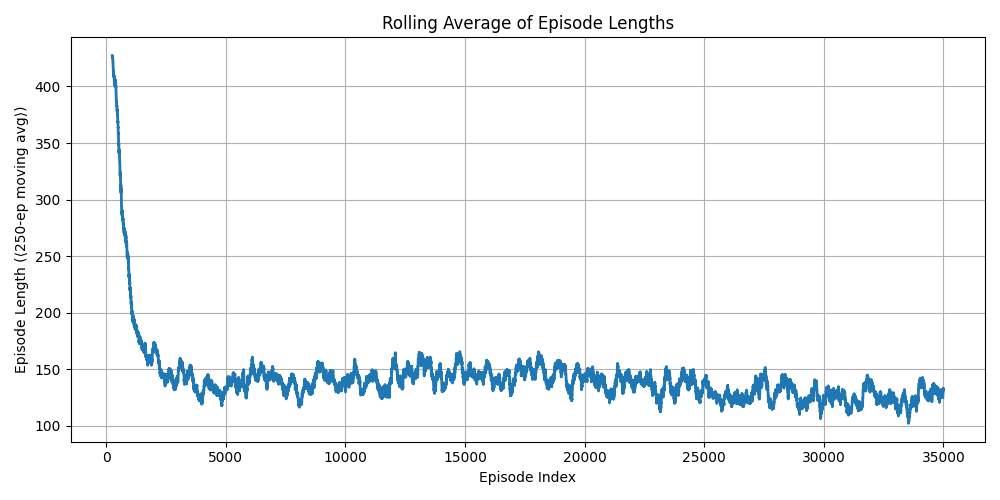
\includegraphics[width=0.9\linewidth]{Bilder/episode_lengths_rolling.png}
\caption{Mittlere Episodenlänge pro 250 Epochen – Navigation}
\label{fig:navigation_training_curve}
\end{figure}
\subsection{Diskussion}
Das Training im Navigationstask verlief insgesamt stabil und führte zu klaren Fortschritten beim Erlernen einer zielgerichteten Bewegung. Dies liegt unter anderem an der kontinuierlichen und dichten Rewardfunktion, die dem Agenten in jeder Situation ein verwertbares Feedback bietet. Besonders die nicht-lineare Skalierung der Belohnung in Zielnähe erwies sich als hilfreich, da sie das Modell dazu motivierte, auch die letzten Schritte präzise zu planen.

Eine weitere wichtige Anpassung war die Modifikation der Kollisionsstrafe: Anstatt harter Bestrafungen bei Kollisionen wurde eine kontinuierliche Penalty eingeführt, die stärker wird, je näher sich der Agent an eine Wand bewegt. Dies reduzierte deutlich die Zahl der Wandkollisionen im Verhalten des Agenten. Allerdings schlägt sich dieser Effekt kaum bis gar nicht in den aggregierten Metriken nieder – etwa weil die Anzahl der Kollisionen keinen direkten Einfluss auf die Episodendauer hat oder durch andere Lernfortschritte überdeckt wird.

Die klare Zielstruktur und die stets verfügbaren Hilfsvektoren (Richtung und Distanz zum Ziel) ermöglichen ein vergleichsweise einfaches Lernen. Allerdings schränkt diese künstliche Unterstützung die Generalisierbarkeit ein – in realitätsnäheren Szenarien wären solche Informationen möglicherweise nicht direkt zugänglich. Eine potenzielle Erweiterung wäre daher, das Training auf rein visuelle Eingaben zu beschränken oder einen gestaffelten Zugriff auf Zielinformationen einzuführen.

\section{Task 2: Exploration}
\label{sec:explore}
\subsection{Methodik}
Task 2 enthält nur eine Futterquelle auf der Karte. Ziel des Agenten ist es, über die leere Karte zu laufen, um das Feld zu finden und es anschließend zu leeren. Der Hilfsvektor ist in dieser Aufgabe nur aktiv, wenn der Agent das Feld im Sichtfeld hat, oder der Agent sich innerhalb eines festgelegten Abstands vom Feld aufhält. Für das Training des Exploretasks wurden iterativ mehrere Modelle mit verschiedenen Rewardfunktionen trainiert.
\begin{figure}[htbp]
  \centering
  \adjincludegraphics[
     width=0.9\linewidth,
     Clip={0 {0\height} 0 {0.1\height}} 
  ]{Bilder/explore.png}
  \caption{Exploration}
  \label{fig:explore_scenario}
\end{figure}

\subsection{Varianten}
\begin{table}[h]
  \centering
  \caption{Reward-Varianten im Explore-Task}
  \begin{tabular}{@{}lll@{}}
    \toprule
    Kürzel & Besondere Reward-Komponente & Motivation \\ \midrule
    V1 & $\Delta$ Distanz zum Feld + gesammeltes Futter & Bewegung zum Feld  \\
    V2 & $\Delta$ Distanz zum Feld wenn in Sicht + Futter & Vermeidung irrelevanter Signale\\
    V3 & V2 + Shaping für Erkundung      & Sparse-Reward-Problem  \\ 
    V4 & V3 mit angepassten Shaping-Parameterm & Optimierung
    \\ \bottomrule
  \end{tabular}
\end{table}

Die ersten Modelle wurden für das verringern der Distanz zum Feld belohnt. Hierbei wurde die Differenz der Distanz $D_t$ zum Feld zur Distanz $D_t-1$ verwendet. Ebenfalls erhält der Agent eine Belohnung, wenn Futter gesammelt wird, er sich also auf dem Feld befindet. In Variante 2 wird die Distanzreward nur gegeben, wenn der Agent das Feld im Sichtfeld hat oder sich innerhalb eines Mindestabstands vom Feld aufhält. In Variante 3 wurde zusätzlich zur Reward in Variante 2 eine Belohnung für das Erkunden der Karte gegeben. Hierbei wurde die Karte in Unterabschnitte unterteilt und der Agent für das Besuchen jedes Kartenabschnittes belohnt. Die Reward auf jedem Unterabschnitt nimmt exponentiell ab, bis sie nach einer bestimmten Anzahl an Schritten auf dem Feld eine linear steigende negative Reward gibt. Dies soll dazu führen, dass der Agent mehrere Felder abläuft, auf diesen aber nicht zu lange verweilt. Für das Training mit Variante 4 wurden die Parameter der Explorationsreward angepasst, indem die Größe der Unterabschnitte variiert wurde. Dies sollte das Erkunden der Karte weiter anregen.

\subsection{Ergebnisse}
\begin{figure}[htbp]
  \centering
  \adjincludegraphics[
     width=0.8\linewidth,
     Clip={0 {0\height} 0 {0.06\height}} 
  ]{Bilder/explore_comparison.jpg}
  \caption{Trainingsverlauf nach Rewardfunktion - Exploration}
  \label{fig:normalized_learning_curves_explore}
\end{figure}
Abbildung ~\ref{fig:normalized_learning_curves_explore} zeigt die normalisierten Rewards während des Trainings der jeweiligen Modelle. \emph{windowed} zeigt dabei jeweils die über Fenster von 25.000 Schritten gemittelten und anschließend normalisierten Rewards. \emph{trend} verwendet über 11 dieser Werte einen gleitenden Durchschnitt, um eine geglättete Trendkurve zu zeigen. Das mit Variante 1 trainierte Modell zeigt direkt anfangs eine kleine Verbesserung, landet danach allerdings in einem Plateau und zeigt keine weitere Verbesserung. Variante 2 zeigt zunächst eine vergleichbare Leistungssteigerung wie Variante 3 und 4, stagniert jedoch frühzeitig und weist im weiteren Verlauf sogar eine systematische Verschlechterung auf. Der Trainingsverlauf geht zum Ende des Trainings wieder leicht nach oben, liegt aber immer noch weiter unter der Performance von Varianten 3 und 4. Diese beiden Modelle zeigen ähnliche Lernkurven, bei denen beide zunächst starke Verbesserungen zeigen, und danach weiter langsam die Ergebnisse stabil verbessern. Die Endperformance von Variante 4 übertrifft die von Variante 3 leicht. Zwar zeigte letztere zu Beginn des Trainings schnellere Fortschritte, diese flachten im weiteren Verlauf jedoch deutlich ab, sodass sie letztlich geringfügig hinter der Nachfolgevariante zurückbleibt.

\subsection{Diskussion}
Das Training im Explore-Task zeigte sich sehr instabil, was letztlich auch zu einer insgesamt schwachen Performance führte. Trotz verschiedener Rewardvarianten konnte kein Modell konsistent lernen das Feld zuverlässig zu finden und zu leeren. Hauptgrund dafür ist die starke Sparsity des Rewards: Belohnung wird nur bei Sichtkontakt oder direkter Nähe zum Feld erteilt – ein Zustand, der ohne zusätzliche Struktur selten eintritt.

Ergänzende Shapingkomponenten wie weitere Erkundungsbelohnungen oder das Belohnen der ersten Sichtung des Felden zeigten nur begrenzte Wirkung. Der Agent blieb häufig entweder vollkommen stehen und lief nur auf zufällig nahegelegene Felder, oder rannte mit voller Geschwindigkeit über die Karte und ignorierte die Felder vollständig. Dies zeigt deutlich, das der Agent die Aufgabenteilung \emph{Feld finden} und \emph{Feld leeren} nur kaum vereinbaren konnte.

Eine sinnvolle Weiterentwicklung wäre der Einsatz von intrinsischer Motivation (zum Beispiel durch curiosity-driven learning) oder hierarchischen Policies, bei denen ein übergeordneter Agent Explorationsziele vorgibt. Zudem wäre eine alternative Evaluation sinnvoll, etwa die Erfolgsdefinition über das erstmalige Erreichen des Feldes, statt über das vollständige Leeren.

\section{Task 3: Fleeing}
\label{sec:flee}
\subsection{Methodik}
Task 3 beinhaltet neben ein paar Hindernissen einen Jäger-Agenten, der gezielt auf den Beute-Agenten zusteuert. Ziel des Agenten ist es, dem Jäger so lange wie möglich zu entkommen. Belohnt wird hier das Vergrößern der Distanz zum Jäger sowie die bisher überlebte Zeit. Die Belohnung wird bewusst verzögert aktiviert, um passives Verhalten zu Beginn der Episode zu vermeiden. Da der Jäger initial in einer bestimmten Entfernung erscheint, würde eine sofortige Überlebensbelohnung dazu führen, dass der Agent ohne aktives Ausweichverhalten belohnt wird. Nach dieser Verzögerung steigt die Überlebensbelohnung langsam bis zu einem Schwellwert an. Als Hilfsvektor erhält der Agent hier die Richtung sowie die Distanz zum Jäger. Mehrere Varianten der Umgebungskonfiguration wurden getestet, darunter Szenarien mit und ohne Fluss sowie mit unterschiedlich großen Hindernissen. Zum Vergleich dieser Einstellungen wurden jeweils separate Modelle trainiert und anschließend evaluiert.
\begin{figure}[htbp]
  \centering
  \adjincludegraphics[
     width=0.9\linewidth,
     Clip={0 {0\height} 0 {0.1\height}} 
  ]{Bilder/flee.png}
  \caption{Flucht}
  \label{fig:flee_scenario}
\end{figure}
\subsection{Ergebnisse}
Abbildung \ref{fig:episode_lengths} zeigt den Mittelwert der Episodenlängen über den Trainingsverlauf der Modelle, die mit unterschiedlichen Hindernissen trainiert wurden. Es ist zu erkennen, dass alle drei Modelle im Laufe des Trainings zunehmend länger überleben, indem sie dem Jäger effektiver entkommen. In den Graphen treten mehrfach temporäre Plateaus auf, die nach weiterem Training jedoch jeweils wieder überwunden werden. Gegen Ende des Trainings liegen die Überlebensdauern des „Medium Rocks“- und des „River“-Modells auf ähnlichem Niveau, während das „Big Rocks“-Modell eine deutlich höhere durchschnittliche Episodenlänge erreicht.

Dabei ist zu beachten, dass die Schwierigkeit der Szenarien unterschiedlich ausfällt, da sie stark von der Navigationslogik des Jägers abhängt: Schon zu Beginn des Trainings weist das River-Szenario eine höhere Überlebensdauer auf, weil der Jäger eine größere Distanz überwinden muss. Trotzdem fällt die Verbesserung gegenüber der Baseline beim River-Modell sehr gering aus und bleibt insgesamt auf niedrigerem Niveau. Im Gegensatz dazu starten beide Fels-Szenarien (mittelgroße vs. große Hindernisse) mit ähnlich niedrigen Baselines, zeigen nachfolgend jedoch einen deutlich stärkeren Leistungszuwachs.
\begin{figure}[htbp]
  \centering
  \adjincludegraphics[
     width=0.8\linewidth,
  ]{Bilder/ep_lengths.jpg}
  \caption{Mittlere Episodenlänge pro 250 Epochen – Flucht}
  \label{fig:episode_lengths}
\end{figure}

Um die Performance der Modelle unabhängiger testen zu können, wurden diese in einem einheitlichen Environment erneut getestet. Dieses Environment enthält sowohl einen Fluss als auch mehrere kleine Steine, was dem Hindernissaufbaue des Survival-Tasks (\ref{sec:survival}) entspricht. Die Tabelle~\ref{tab:survival_comparison} zeigt die durchschnittliche Überlebensdauer der jeweiligen Modelle, berechnet über 1000 Episoden in der beschriebenen Umgebung. Hierbei zeigt sich, dass das Modell aus dem Fluss-Szenario schlechter abschneidet, obwohl dieses dem getesteten Aufbau ähnlicher ist als die anderen beiden Environments. Das „Medium Rocks“-Modell zeigt hierbei die beste Performance, während die Leistung des „Big Rocks“-Modells leicht unter der des „River“-Modells liegt.

\begin{table}[h]
  \centering
  \caption{Überlebensdauer im Survival-Task}
  \begin{tabular}{@{}l c@{}}
    \toprule
    Trainingsszenario &
      \multicolumn{1}{c}{durchschnittliche Überlebensdauer} \\ \midrule
    große Steine   & $71,6 \pm 1,5$ \\
    mittelgroße Steine  & $89,4 \pm 2,1$ \\
    Fluss          & $78,4 \pm 1,8$ \\ 
    \bottomrule
  \end{tabular}
  \label{tab:survival_comparison}
\end{table}


\subsection{Diskussion}
Die Ergebnisse aus Tabelle \ref{tab:survival_comparison} verdeutlichen, dass die Übertragbarkeit der Subtask-Modelle in das einheitliche Test-Environment nicht allein durch die strukturelle Ähnlichkeit des Trainingsszenarios erklärt werden kann. Obwohl das River-Modell dem Aufbau der Testumgebung am ähnlichsten ist, erreicht es eine geringere Überlebensdauer als die des Modells, welches mit kleinen Hindernissen trainiert wurde. Dies deutet darauf hin, dass der erhöhte Abstand zum Jäger im Fluss-Szenario zwar initial das Überleben erleichtert, aber keine robusten Ausweichstrategien fördert. 

Im Gegensatz dazu mussten die Agenten im „Medium Rocks“-Szenario von Beginn an komplexere Routen um Hindernisse planen und adaptiv auf enge Passagen reagieren. Diese stärkere Navigationsanforderung scheint zu allgemeineren und effizienteren Taktiken geführt zu haben, die sich auch im neuen Environment bewähren. 

Die unterschiedlichen Schwierigkeitsgrade der Trainingsszenarien können die absoluten Überlebenszeiten verzerren. Entscheidend ist jedoch, dass das „Medium Rocks“-Modell, trotz des anspruchsvolleren Settings, am stärksten von seinem Training profitiert und die höchsten Überlebenswerte erzielt. Insgesamt legt dies nahe, dass eine höhere Komplexität im Subtask-Training hier die Generalisierungsfähigkeit verbessert und zu nachhaltigeren Fluchtstrategien führt.


\section{Task 4: Survival}
\label{sec:survival}
\subsection{Methodik}
Dieser Task beschreibt das eigentliche Endziel, welches das Modell erreichen soll. In diesem Environment hat der Agent die Aufgabe, eine Futterquelle zu finden und zu leeren, bevor er vom Jäger gefressen wird. Er erhält als Hilfsvektoren sowohl die Richtung und Distanz zum Jäger, als auch die Richtung und Distanz zum Feldstück, wenn er dieses in seinem Sichtfeld hat. 
\begin{figure}[htbp]
  \centering
  \adjincludegraphics[
     width=0.9\linewidth,
     Clip={0 {0\height} 0 {0.1\height}} 
  ]{Bilder/full.png}
  \caption{Gesamtszenario}
  \label{fig:full_scenario}
\end{figure}
Da dieses Szenario Komponenten all der Unteraufgaben enthält, wurde zunächst eine Kombination der drei taskspezifischen Rewardfunktionen getestet. Diese Rewardfunktion belohnte somit das Verkleinern der Distanz von sichtbaren Feldabschnitten, das Vergrößern der Distanz zum Jäger, das Vermeiden von Kollisionen, sowie eine Belohnung für längeres Überleben und eine Strafe für eine Kollision mit dem Jäger. Ebenfalls wurde die zeitverzögerte Überlebensbelohnung aus dem Abschnitt~\ref{sec:flee} übernommen. Es wurde ebenfalls eine vereinfachte Rewardfunktion implementiert, um das Training zu stabilisieren und gegenläufige Signale zu vermeiden.

Diese angepasste Rewardfunktion entfernt die gegenläufige Überlebensbelohnung sowie die Penalty für Kollisionen mit Wänden. Ebenfalls fällt die rasterbasierte Erkundungsbelohnung aus Abschnitt~\ref{sec:explore} weg. Somit bleiben eine Penalty für eine Kollision mit dem Jäger und verstrichene Zeit, sowie Belohnungen für das Vergrößern der Distanz zum Jäger, Verringern der Distanz zu sichtbaren Futterquellen sowie das Sammeln von Futter. Um die Änderungen zu kompensieren, wurden die Parameter der bleibenden Rewardkomponenten leicht angepasst.

\subsection{Ergebnisse}
Abbildung ~\ref{fig:task4_learning_curve} zeigt zwei Trainingsabläufe im vollen Environment. Die Modelle wurden jeweils mit den gleichen Parametern, aber unterschiedlichen Rewardfunktionen trainiert. \emph{combined} zeigt hierbei das Modell, welches mit der Kombination der Rewardfunktionen aus den Subtasks trainiert wurde, während \emph{adjusted} die in der Methodik angepasste und vereinfachte Rewardfunktion verwendet. \emph{windowed} zeigt dabei jeweils die über Fenster von 25.000 Schritten gemittelten und anschließend normalisierten Rewards. \emph{trend} verwendet über 11 dieser Werte einen gleitenden Durchschnitt, um eine geglättete Trendkurve zu zeigen. Die kombinierte Rewardfunktion zeigt insgesamt kaum bis gar keinen Lerneffekt, während sich die Performance des Modells mit justierter Rewardfunktion bis Schritt 2.000.000 verbessert, und danach nur leichte Schwankungen zeigt.

\begin{figure}[htbp]
  \centering
  \adjincludegraphics[
     width=0.8\linewidth,
     Clip={0 {0\height} 0 {0.06\height}} 
  ]{Bilder/learning_curves_task4.png}
  \caption{Trainingsverlauf Surival-Task}
  \label{fig:task4_learning_curve}
\end{figure}
\subsection{Diskussion}
Die Überlebensumgebung stellte sich als besonders herausfordernd heraus, da sie mehrere konkurrierende Ziele gleichzeitig verlangt: Nahrung sammeln, Jäger meiden, Karte erkunden und Hindernisse umgehen. Das initiale Rewarddesign, welches die Rewardfunktionen der Subtasks kombinierte, führte hierbei zu instabilen Lernverläufen. Insbesondere widersprüchliche Signale – etwa Überlebensbelohnung bei gleichzeitigem Ignorieren von Nahrung – verhinderten eine kohärente Strategieentwicklung.

Die vereinfachte Rewardfunktion reduzierte diese Konflikte, was sich in einer deutlich verbesserten Lernkurve widerspiegelte. Hierbei zeigte sich, dass klare, priorisierte Ziele (beispielsweise Nahrungssuche und Flucht mit klaren Bedingungen) besser vom Modell internalisiert werden als komplexe, gleichgewichtete Rewardmischungen. Diese Erkenntnis unterstreicht die Bedeutung einer sorgfältigen Rewardabstimmung bei Multi-Ziel-Szenarien.

\section{Curriculum Learning}
\subsection{Methodik}
\label{sec:methodology}
Der methodische Aufbau zur Untersuchung des Curriculum-Learning-Ansatzes basiert auf dem Vergleich unterschiedlicher Trainingsstrategien. Curriculum Learning bezeichnet eine Strategie, bei der das Training komplexer Modelle schrittweise anhand von zunehmend anspruchsvolleren Aufgaben durchgeführt wird, beginnend mit einfachen Teilaufgaben und schrittweise übergehend in komplexere Szenarien. Konkret wurde hierzu der Trainingsverlauf eines vollständig neu initialisierten Modells mit den Verläufen der Modelle verglichen, deren Gewichte zuvor in den spezifischen Subtasks (Navigation, Exploration, Fleeing) vortrainiert worden waren.

Dazu wurden die jeweils besten Modelle aus den vorhergehenden Subtasks nach dem initialen Training erneut geladen und anschließend im Überlebensszenario weitertrainiert. Ziel dieses Vorgehens war es, zu untersuchen, ob durch das Vortrainieren in vereinfachten Umgebungen eine schnellere Konvergenz oder eine verbesserte finale Performance in der komplexen Gesamtumgebung erzielt werden kann. 

Durch den direkten Vergleich der Lernkurven zwischen neu initialisierten und vortrainierten Modellen konnte somit evaluiert werden, ob der Curriculum-Learning-Ansatz zu signifikanten Vorteilen hinsichtlich der Lerngeschwindigkeit und Qualität der gelernten Strategien führt.\subsubsection*{Bezeichnungen der Modellklassen}
Im Folgenden werden vier Modellklassen unterschieden:
\begin{itemize}
  \item Modelle, die im Navigation-Task vortrainiert und anschließend in der vollständigen Umgebung weiter trainiert wurden, werden \emph{Navigationsmodelle} genannt.
  \item Modelle, die im Exploration-Task vortrainiert und anschließend in der vollständigen Umgebung weiter trainiert wurden, werden \emph{Explorationsmodelle} genannt.
  \item Modelle, die im Fleeing-Task vortrainiert und anschließend in der vollständigen Umgebung weiter trainiert wurden, werden \emph{Fluchtmodelle} genannt.
  \item Frisch initialisierte Modelle, die ohne Vortraining direkt in der Zielumgebung trainiert werden, werden \emph{Scratch-Modelle} genannt.
\end{itemize}
Die Scratch-Modelle besitzen keine vortrainierten Gewichte und werden ausschließlich im vollständigen Szenario von Grund auf trainiert.  

Um dabei einen fairen Vergleich der Trainingsabläufe zu gewährleisten, wurden beim Transfertraining ausschließlich die Modellgewichte geladen, der Optimizer jedoch neu initialisiert. Dies stellt sicher, dass alle getesteten Modelle die gleiche Ausgangsbasis hinsichtlich der Lernrate und weiterer Optimizer-spezifischer Parameter besitzen.


\subsubsection{Evaluierung}
Die Evaluierung der Performance im Environment erfolgte mithilfe mehrerer speziell definierter Metriken. Wichtig sind hierbei unter anderen die Menge des gesammelten Futters, die durchschnittliche Überlebensdauer sowie die durchschnittliche Zeit bis zum vollständigen Leeren eines Feldes.

Bei der Berechnung der jeweiligen Metriken werden nur jene Episoden berücksichtigt, die die entsprechende Voraussetzung erfüllen. Konkret bedeutet dies, dass Episoden, in denen der Agent vom Jäger gefressen wird, ausschließlich zur Ermittlung der durchschnittlichen Überlebensdauer herangezogen werden. Episoden, die erfolgreich mit einem vollständig geleerten Feld enden, werden hingegen für die Berechnung der Zeit-zu-Futter-Metrik genutzt.
 
Diese Aufteilung spielt ebenfalls eine Rolle bei der Berechnung der Erfolgsrate. Als erfolgreich gelten Episoden, in denen der Agent das Feld vollständig leert. Alle anderen Episoden werden als gescheitert gewertet. Die Erfolgsrate gibt somit den Anteil erfolgreicher Episoden an der Gesamtzahl der Evaluierungsepisoden in Prozent an.

Um diese Metriken zu ermitteln, absolvieren jeweils alle drei Modelle aus den vier Gruppen insgesamt 1000 Episoden im Überlebensszenario. Diese Episoden sind für alle Modelle identisch und wurden von keinem der Modelle während des Trainings zuvor gesehen. Die daraus resultierenden Werte werden anschließend gruppenweise zusammengefasst und ausgewertet.

\subsection{Ergebnisse}
\subsubsection{Trainingsverlauf}
Abbildung~\ref{fig:normalized_rewards} zeigt die Trainingsverläufe der in den Subtasks vortrainierten Modelle im Vergleich zum Scratch-Modell. Die dargestellten Werte entsprechen jeweils den Mittelwerten aus drei Trainingsdurchläufen.
\begin{figure}[htbp]
  \centering
  \adjincludegraphics[
     width=0.9\linewidth
  ]{Bilder/learning_curves.png}
  \caption{Trainingsverlauf Curriculum Learning}
  \label{fig:normalized_rewards}
\end{figure}
Zu Beginn des Trainings zeigen die Scratch-Modelle eine schnelle Verbesserung der Performance, erreichen jedoch nach ungefähr der Hälfte des Trainingsverlaufs ein Plateau, auf welchem sich die Leistung nur geringfügig weiter verbessert.

Im Vergleich dazu weisen die Fluchtmodelle eine deutlich flachere Lernkurve auf, was darauf hindeutet, dass diese Modelle zunächst Schwierigkeiten hatten, zusätzliche relevante Strategien (wie das Sammeln von Futter) zu integrieren, nachdem sie zuvor hauptsächlich auf Fluchtstrategien trainiert wurden. Trotz ihres langsameren Fortschritts erreichen die Fluchtmodelle am Ende des Trainings ein ähnliches Performance-Niveau wie die Scratch-Modelle.

Die Navigationsmodelle starten hingegen mit einem deutlich höheren Grundniveau, was darauf hinweist, dass diese bereits relevante Fähigkeiten zur Orientierung und Zielnavigation internalisiert haben. Nach einer schnellen anfänglichen Anpassungsphase erreichen diese Modelle jedoch ebenfalls ein ähnliches Plateau wie die zufällig initialisierten Modelle.

Die Explorationsmodelle zeigen zunächst eine instabilere und insgesamt niedrigere Lernkurve. Allerdings übertreffen diese gegen Ende des Trainingszeitraums leicht die Performance der anderen Modelle. Dies deutet darauf hin, dass die explorativen Fähigkeiten erst im späteren Trainingsverlauf einen Vorteil bieten, nachdem die Agenten gelernt haben, diese Fähigkeiten effizient in die Gesamtstrategie zu integrieren.


\subsubsection{Performance}
Obwohl die Modelle hinsichtlich der Gesamtbelohnung am Ende des Trainings ähnliche Niveaus erreichen, erfasst dieser Wert nicht vollständig alle relevanten Aspekte des Agentenverhaltens. Da die eingesetzte Rewardfunktion unterschiedliche Verhaltensweisen gleichzeitig belohnt, kann ein ähnlich hohes Gesamtrewardniveau unterschiedliche Strategien verschleiern, welche die Modelle jeweils bevorzugen. Um eine differenzierte Bewertung der Performance zu ermöglichen, ist es deshalb notwendig, einzelne Komponenten des Verhaltens separat zu analysieren.
\begin{figure}[htbp]
  \centering
  \adjincludegraphics[
     width=0.6\linewidth
  ]{Bilder/total_food_collected_bar_median.png}
  \caption{Futter pro Episode (median)}
  \label{fig:food_per_episode}
\end{figure}
Abbildung~\ref{fig:food_per_episode} zeigt den Median der Menge an Futter, welches die jeweiligen Modelle in der im Methodikabschnitt ~\ref{sec:methodology} beschriebenen Evaluation gesammelt haben \footnote{Der Median wird aufgrund der hohen Zahl an Ausreißern im Fluchtmodell verwendet, die durch das Nachwachsen des Futters entsteht. Der Agent sammelt so zwar mehr Futter, was aber nicht zwangsläufig zum besseren erfüllen der Aufgabe führt}. Hierbei zeigt sich eine positive Tendenz für die Explorationsmodelle, was sich mit den Erkenntnissen der Trainingsverläufe deckt. Ebenfalls zeigen die Scratch-Modelle insgesamt die schlechteste Performance, während Navigations- und Fluchtmodelle ähnliche Werte aufweisen. Insgesamt zeigen jedoch alle Modelle ähnliche Performance in diesem Bereich.
\newpage

Ebenfalls relevant zu dieser Metrik ist die Betrachtung der Zeit die ein Agent benötigt, um das Feld vollständig zu leeren - ein Agent kann das Feld nach 10 oder nach 100 Schritten vollständig leeren und die gleiche Menge an Futter erhalten.
\begin{figure}[htbp]
  \centering
  \adjincludegraphics[
     width=0.6\linewidth
  ]{Bilder/time_to_goal_bar_se.png}
  \caption{Zeit zu geleertem Feld}
  \label{fig:time_to_goal}
\end{figure}
Hierbei zeigt sich deutlich, dass die Fluchtmodelle länger als die anderen Modelle brauchen, um das Feld zu erreichen und dieses zu leeren. Die Navigations-, Explorations- und Scratch-Modelle zeigen hierbei eine ähnliche Leistung auf.

Episoden, in denen das Feld nicht geleert wurde, fallen stattdessen in die Metrik zur Lebensdauer der Agenten, welche in Abbildung~\ref{fig:time_alive} zu sehen ist.
\begin{figure}[htbp]
  \centering
  \adjincludegraphics[
     width=0.7\linewidth
  ]{Bilder/time_alive_bar_se.png}
  \caption{Lebensdauer}
  \label{fig:time_alive}
\end{figure}
Hierbei zeigt sich eine ähnliche Tendenz zu der in Abbildung~\ref{fig:time_to_goal}, wobei Fluchtmodelle länger überleben. Die anderen Modellarten zeigen hierbei wieder ähnliche Performance, während die Scratch-Modelle hier eine leicht geringere Überlebensdauer aufweisen.

Um die vorherigen beiden Metriken jedoch korrekt einordnen zu können ist ebenfalls die Betrachtung der Erfolgsrate nötig. In der Regel endet eine Episode, weil entweder das gesamte Feld geleert wurde oder weil der Agent von einem Jäger getroffen wurde. Theoretisch existiert noch ein dritter Fall, bei dem keine dieser beiden Bedingungen zutrifft und die Episode durch Erreichen der maximalen Episodenlänge beendet wird. Dieser Fall tritt jedoch sehr selten auf und wurde daher in den bisherigen Metriken der Kategorie Überlebensdauer zugeordnet.

In Abbildung~\ref{fig:succesrate} zählen alle Episoden, die mit einem geleerten Feld enden, als erfolgreich beendet, während alle anderen Episoden als gescheitert gelten. Hier wird deutlich, dass die Explorationsmodelle die beste Leistung besitzen. Die Navigationsmodelle zeigen ebenfalls eine kleine Verbesserung gegenüber den Scratch-Modellen auf, während die Fluchtmodelle schlechter abschneiden. Diese Diskrepanz zu den gesammelten Futterwerten, die in Abbildung~\ref{fig:food_per_episode} gezeigt werden, entsteht durch das Implementierte nachwachsen des Futters. Die Agenten sammeln also alle grob die gleiche Menge an Futter, allerdings scheinen die Explorationsmodelle gezielter auf dem Feld zu warten und es vollständig zu leeren, während die Fluchtmodelle dieses zwar betreten, es allerdings auch schnell wieder verlassen um gegebenenfalls später zurückzukehren. Somit ergibt sich eine ähnliche Menge an gesammeltem Futter mit unterschiedlicher Erfolgsrate.

\begin{figure}[htbp]
  \centering
  \adjincludegraphics[
     width=0.6\linewidth
  ]{Bilder/successful_comparison.png}
  \caption{Anteil erfolgreich beendeter Episoden}
  \label{fig:succesrate}
\end{figure}
\subsection{Diskussion}

Die Evaluation des Curriculum-Learning-Ansatzes zeigte, dass vortrainierte Modelle nicht nur schneller lernen, sondern auch spezialisierte Verhaltensweisen beibehalten – mit teils positiven, teils negativen Folgen. Besonders die Navigationsmodelle profitierten stark vom Vortraining, indem sie zu Beginn schneller das Zielverhalten lernten. Die Explorationsmodelle zeigten erst später Vorteile, entwickelten jedoch eine höhere Erfolgsrate. Dagegen hatten die Fluchtmodelle Schwierigkeiten, ihr Fluchtverhalten mit der Nahrungssuche zu kombinieren, was auf negative Interferenz hinweist.

Diese Beobachtungen zeigen, dass Transferlernen nicht nur Vorteile bringt, sondern auch bestehende Verhaltensmuster verfestigen kann, die im neuen Kontext suboptimal sind. Denkbar wäre hier ein modularer Aufbau der Policy – etwa durch getrennte Komponenten für Flucht und Nahrung, die situativ gewichtet werden.

\section{Retention nach Full-Task-Fine-Tuning}
Im folgenden Abschnitt wird die Performance der Flucht-, Navigations- und Explorationsmodelle im ursprünglichen Subtask mit der Performance der Baseline-Modelle verglichen. Ziel ist es, zu evaluieren, ob die Modelle die ursprünglich gelernten Fähigkeiten nach dem Full-Task-Fine-Tuning beibehalten haben oder ob diese durch neue Strategien ersetzt beziehungsweise abgeschwächt wurden.

\subsection{Methodik}
Für jeden der drei Subtasks—Explore, Flee und Navigate—wurden zwei Modellvarianten jeweils über 1000 unabhängige Episoden hinweg evaluiert. Die Baseline-Modelle wurden ausschließlich im jeweiligen Subtask trainiert, während die Fine-Tuned-Varianten im Anschluss ein zusätzliches Full-Task-Training erhielten. Als Leistungskennzahlen dienten im Explore-Subtask die durchschnittliche Zeit bis zum Erreichen des Ziels (Time to Goal) und die Erfolgsrate (Success Rate), im Flee-Subtask die mittlere Überlebenszeit in Schritten (Time Alive) und im Navigate-Subtask sowohl die Time-to-Goal als auch die Clear Rate, definiert als Anteil der Episoden, in denen das Ziel erreicht wurde.

\subsection{Ergebnisse}

\paragraph{Explore}
Nach dem Full-Task-Fine-Tuning zeigt das Explore-Modell eine deutliche Leistungssteigerung.  
Die durchschnittliche \emph{Time-to-Goal} verkürzt sich von $115{,}8 \pm 3{,}5$ auf $104{,}5 \pm 3{,}0$ Schritte\footnote{Angaben jeweils Mittelwert $\pm$ Standardfehler des Mittelwerts.}. Gleichzeitig steigt die Erfolgsrate um fast dreizehn Prozentpunkte auf $94{,}6\%$. Hier ist zu beobachten, dass der Agent die Futterquellen nicht nur schneller findet, sondern diese auch konsistenter vollständig leert. 

\begin{table}[H]
  \centering\footnotesize
  \setlength{\tabcolsep}{4pt}
  \caption{Retention im Explore-Subtask}
  \begin{tabular}{@{}lcc@{}}
    \toprule
    Modell                     & Time to Goal & Success Rate \\
                               & [Steps]      & [\%]         \\ 
    \midrule
    Explore-only               & $115{,}8 \pm 3{,}5$ & $81{,}7$  \\
    Explore \(\rightarrow\) Survival & $104{,}5 \pm 3{,}0$ & $94{,}6$  \\
    \bottomrule
  \end{tabular}
\end{table}

\paragraph{Flee}
Im Flee-Subtask sinkt die mittlere Überlebenszeit und damit die Performance nach dem Full-Task-Training von $149{,}4 \pm 20$ auf $115{,}1 \pm 2{,}6$ Schritte. 
\begin{table}[H]
  \centering\footnotesize
  \setlength{\tabcolsep}{4pt}
  \caption{Retention im Flee-Subtask}
  \begin{tabular}{@{}lc@{}}
    \toprule
    Modell                     & Time Alive  \\ 
                                & [Steps]   \\ 
    \midrule
    Flee-only                  & $149{,}4 \pm 3{,}3$    \\
    Flee \(\rightarrow\) Survival    & $115{,}1 \pm 2{,}6$  \\
    \bottomrule
  \end{tabular}
\end{table}

\paragraph{Navigate}
Die Time-to-Goal im Navigate-Subtask ist relativ stabil und steigt nach dem Survival-Fine-Tuning von $139 \pm 3{,}3$ auf $142{,}1 \pm 3{,}7$ Schritte, während die Clear Rate wiederum von $95{,}5\%$ auf $90{,}6\%$ abnimmt. Beide Modelle zeigen teilweise Probleme, die letzten Schritte in Richtung des Ziels zu machen um dieses zu erreichen. 
\begin{table}[H]
  \centering\footnotesize
  \setlength{\tabcolsep}{4pt}
  \caption{Retention im Navigate-Subtask}
  \begin{tabular}{@{}lcc@{}}
    \toprule
    Modell                     & Time to Goal & Clear Rate  \\
                               & [Steps]      & [\%]        \\ 
    \midrule
    Navigate-only              & $139 \pm 3{,}3$   & $95{,}5$  \\
    Navigate \(\rightarrow\) Survival & $142{,}1 \pm 3{,}7$ & $90{,}6$  \\
    \bottomrule
  \end{tabular}
\end{table}

\subsection{Diskussion}
Die Retention-Analyse illustriert ein differenziertes Spannungsfeld zwischen \emph{Stabilität} bereits gelernter Teilstrategien und der \emph{Anpassungsfähigkeit} an das komplexere Gesamtszenario:


\paragraph{Explore}  
Im Explore-Subtask verbessert sich der Agent deutlich: Er erreicht das Ziel fast zehn Prozent schneller, und die Erfolgsrate steigt von gut 82\% auf knapp 95\%. Das Fine-Tuning mit permanentem Jägerdruck motiviert den Agenten, die Karte systematischer abzulaufen, anstatt sich auf zufällige Bewegungen zu verlassen. Damit wird die ursprüngliche „blinde“ Exploration zu einem zielgerichteten Suchverhalten verfeinert, das Sichtkontakt rascher in konkrete Sammelaktionen umsetzt.

\paragraph{Flee}  
Die Fluchtfähigkeiten verschlechtern sich hingegen erheblich; die mittlere Überlebenszeit sinkt um fast ein Viertel. Eine naheliegende Erklärung ist ein Konflikt in der Belohnungsstruktur: Während des Full-Task-Trainings konkurrieren positive Signale für Futteraufnahme mit denen für Distanz zum Jäger. Das neu gewichtete Sammelziel verdrängt dabei Teile der zuvor erlernten Ausweichstrategie. Hinzu kommt, dass der Agent im Full-Task zwangsläufig häufiger riskante Positionen nahe am Jäger aufsucht, weil viele Futterquellen in offenen Bereichen liegen. Dadurch verschiebt sich die Zustandsverteilung des Trainingsverhalten, das im reinen Flee-Benchmark sofort bestraft wird, im Gesamtumfeld jedoch oft ohne negative Konsequenz bleibt. 

\paragraph{Navigation}  
Die Navigationsleistung bleibt auch nach dem Full-Task-Fine-Tuning nahezu unverändert. Die leichte Zunahme der \emph{Time to Goal} um gut zwei Schritte ist vernachlässigbar und deutet auf ein bereits hohes Ausgangsniveau hin, wie in Abbildung~\ref{fig:normalized_rewards} zu erkennen ist. Offenbar ist die vorhandene Pfadplanungsheuristik auch im erweiterten Szenario ausreichend, da zusätzliche Anforderungen wie das Ausweichen vor Jägern oder die Nahrungsaufnahme nur geringe strukturelle Anpassungen der Policy erfordern.